\documentclass[../zavrsni.tex]{subfiles}

\begin{document}

\sloppy

\justifying

Postupkom opisanim u prošlom poglavlju generirani su izvještaji za ranije opisane algoritme koji su implementirani unutar FreeRTOS-a.
Iz izvještaja je potrebno dobiti grafove, kako bi se vizualizirali i lakše interpretirali dobiveni rezultati. 
Za to je korišten programski jezik Python i u njemu uključen paket za crtanje grafičkih prikaza \texttt{matplotlib}. 
Sve simulacije su za određene uvjete pokrenute 20 puta, pa je zbog toga na grafovima prikazan prosjek dobivenih rezultata. 

Za početak će biti prikazani rezultati simulacija algoritma EDF. Graf koji prikazuje kvalitetu usluge u odnosu na faktor opterećenja 
prikazan je na slici 5.1. 
\begin{figure}[!htb]
    \center{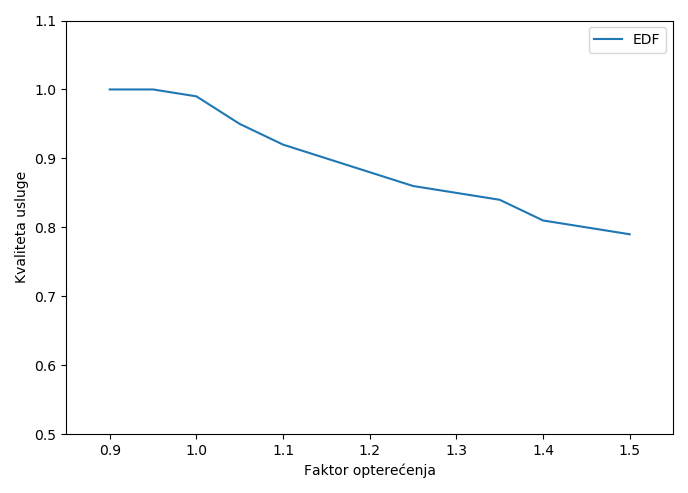
\includegraphics[width=\textwidth]
    {images/Figure_3.png}}
    \caption{\label{fig:my-label} Kvaliteta usluge algoritma EDF}
\end{figure}
Algoritam EDF je izdvojen od ostala dva jer nije primjenjiv za ublaženo-stroge
uvjete u sustavima za rad u stvarnom vremenu. Stoga je uz kvalitetu usluge, na posebnom grafu na slici 5.2 prikazan odnos broja kršenja 
postavljenih uvjeta u skip over modelu i ukupnog broja zadataka. Kršenje ublaženo-strogih uvjeta prikazuje se relativno u odnosu na broj 
poslova jer svaka simulacija ima različite vrijednosti perioda, a time i različit broj poslova.
Može se uočiti da porastom opetrećenja sustava, raste broj prekršenih uvjeta postavljenih nad skupom zadataka.

\begin{figure}[!htb]
    \center{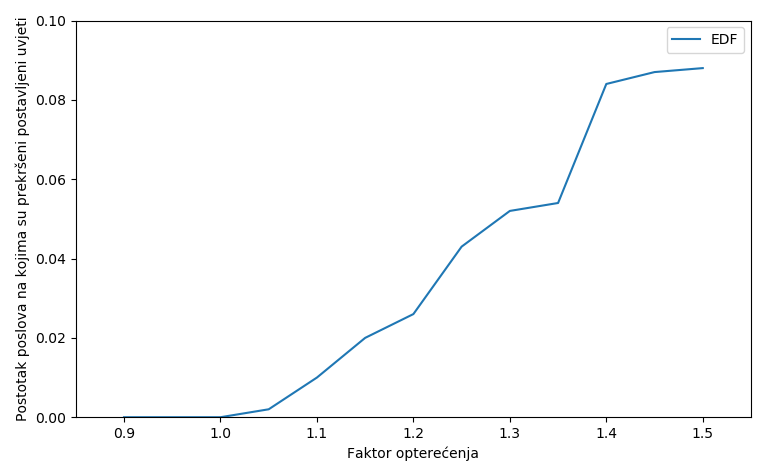
\includegraphics[width=\textwidth]
    {images/poseban.png}}
    \caption{\label{fig:my-label} Postotak poslova na kojima je prekršen postavljen ublaženo strogi uvjet}
\end{figure}

U kontekstu skip-over modela ublaženo-strogih uvjeta potrebno je usporediti algoritme RTO i BWP. Graf dobiven iz podataka skupljenih simulacijama
prikazan je na slici 5.3. Na grafu je prikazana ostvarena kvaliteta usluge u ovisnosti o faktoru opeterećenja.  
Vidljivo je da BWP algoritam za mala 
opterećenja ima puno veću kvalitetu usluge, koja opada kako opterećenje sustava raste. Kod algoritma RTO kvaliteta usluge je gotovo nepromjenjiva
u odnosu na faktor opterećenja i znatno niža od one kod algoritma BWP. 

\begin{figure}[!htb]
    \center{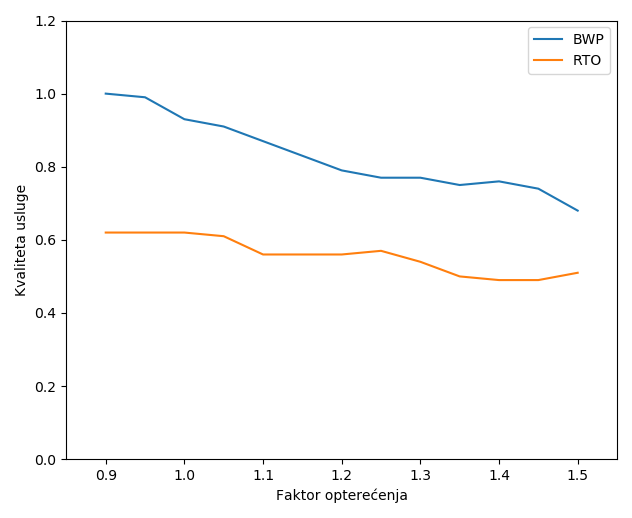
\includegraphics[width=\textwidth]
    {images/Figure_2.png}}
    \caption{\label{fig:my-label} Usporedba algoritama BWP i RTO}
\end{figure}

\end{document}